\documentclass[usenames,dvipsnames]{beamer}

\usepackage{tikz}
\usepackage{tkz-berge}
\usepackage{tkz-graph}
\usepackage{subcaption}

\usetikzlibrary{patterns,arrows,decorations.pathreplacing}

\usepackage{xcolor}
\definecolor{dblue}{RGB}{20,66,129}
\definecolor{rose}{RGB}{255,101,122}
\definecolor{crimsonred}{RGB}{132,22,23}
\definecolor{darkblue}{RGB}{72,61,139}

\definecolor{deepblue}{RGB}{36,123,160}
\definecolor{deepred}{RGB}{255,22,84}
\definecolor{deeporange}{RGB}{240,111,62}

\definecolor{olive}{rgb}{0.3, 0.4, .1}
\definecolor{fore}{RGB}{249,242,215}
\definecolor{back}{RGB}{51,51,51}
\definecolor{title}{RGB}{255,0,90}
\definecolor{dgreen}{rgb}{0.,0.6,0.}
\definecolor{gold}{rgb}{1.,0.84,0.}
\definecolor{JungleGreen}{cmyk}{0.99,0,0.52,0}
\definecolor{BlueGreen}{cmyk}{0.85,0,0.33,0}
\definecolor{RawSienna}{cmyk}{0,0.72,1,0.45}
\definecolor{Magenta}{cmyk}{0,1,0,0}


\title{Fractals avoiding Fractal Sets}
\author{Jacob Denson}
\institute{University of British Columbia}

\begin{document}

\maketitle

\begin{frame}
  \frametitle{Pattern Avoidance Problems}

\begin{tabular}{p{0.8\textwidth}p{0.3\textwidth}}

\begin{itemize}
    \item How large can the Hausdorff dimension of a $\mathbf{Q}$ vector subspace of $\mathbf{R}^n$ be not containing any points in $\mathbf{Q}^n$.

     \pause
     \item What is the largest Hausdorff dimension of a subset of $\mathbf{R}^d$ such that the distances between any two points is irrational?

     \pause
     \item Given any equation $f$, what is the largest Hausdorff dimension of $X \subset \mathbf{R}^d$ such that for any distinct $x_1, \dots, x_n \in X$, $f(x_1, \dots, x_n) \neq 0$. 
\end{itemize}

\end{tabular}

\end{frame}

\begin{frame}
    \frametitle{Two Observations}

    \begin{itemize}
        \item Problems can be summarized as finding $X$ such that $X^n$ avoids a given set $Z$, except for `repeated coordinate points'. Let
        \[ \Delta = \{ x \in (\mathbf{R}^d)^n: x_i = x_j\ \text{for distinct}\ i,j \in \{ 1, \dots, n \} \} \]
        %
        \vspace{-1.5em}

%            \begin{center}
%        \begin{tabular}{| c | c |}
%            \hline
%            $Z$ & Pattern Problem\\
%            \hline
%            $\{ (x,y,z) \in \mathbf{R}^3: z - x = 2(y-x) \}$ & $X^3 \cap Z \subset \Delta$ iff $X$ avoids three term arithmetic progressions.\\
%            $\{ (x,y,z,w) \in \mathbf{R}^{4d}: d(x,y) = d(z,w) \}$ & $X^4 \cap Z \subset \Delta$ if and only if the points in $X$ have distinct distances.\\
%            $\{ (x,y,z) \in \mathbf{R}^{3d}: \frac{(x - z) \cdot (y - z)}{|x-z||y-z|} = \cos(120^\circ) \}$ & $X^4 \cap Z \subset \Delta$ if and only if $X$ avoids $120^\circ$ angles.\\
%            \hline
%        \end{tabular}
%        \end{center}

        \begin{itemize}
            \pause
           \item For any $n$, if $Z_n = \{ x \in \mathbf{R}^{nd}: \text{there is}\ a_1, \dots, a_n\ \text{s.t.}\ a_1x_1 + \dots + a_nx_n \in \mathbf{Q} \}$, then $X$ generates a vector space avoiding the rationals if and only if $X^n \cap Z_n \subset \Delta$ for all $n$.

           \pause
            \item If $Z = \{ (x,y): d(x,y) \in \mathbf{Q} \} \subset \mathbf{R}^{2d}$, then points in $X$ have irrational distances if and only if $X^2 \cap Z \subset \Delta$.

            \pause
            \item If $Z = f^{-1}(0)$, $X$ avoids zeroes of $f$ if and only if $X^n \cap Z \subset \Delta$.
        \end{itemize}
    \end{itemize}
\end{frame}

\begin{frame}
    \frametitle{The Generic Problem}

    \begin{itemize}
        \item {\bf Fractal Avoidance Problem}: Given $Z \subset \mathbf{R}^{nd}$, find $X \subset \mathbf{R}^d$ with large Hausdorff dimension such that $X^n \cap Z \subset \Delta$.

        \pause
        \item Math\'{e} (2012): If $Z \subset \mathbf{R}^{nd}$ is an algebraic hypersurface specified by a degree $r$ polynomial in $nd$ variables with rational coefficients, then we can find $X$ solving the fractal avoidance problem for $Z$ with dimension $d/r$. This is independent of $n$.

        \pause
        \item Pramanik and Fraser (2016): If $Z$ is a smooth hypersurface of dimension $nd - d$, we can find $X$ with dimension $d/(n-1)$.
    \end{itemize}
\end{frame}

\begin{frame}
    \frametitle{Increasing the Difficulty$\dots$}

    \begin{center}
     \Huge {\it What if the Patterns are Fractally Specified...}
    \end{center}
\end{frame}

%\begin{frame}
%    \frametitle{The Avoidance Problem}

%        \begin{itemize}

%            \item Our method naturally considers an equivalent setup.

%            \item {\bf Fractal Avoidance Problem}: Given $Y \subset \mathbf{R}^{nd}$, find $X \subset \mathbf{R}^d$ such that $X^n \cap Y \subset \Delta$, where $\Delta = \{ x: x_i = x_j\ \text{for some $i,j$} \}$.

%            \item Equivalent by setting $Y = f^{-1}(0)$, or $f = \mathbf{I}_{Y^c}$.

%            \item Our method only uses the structure of the zero set, not $f$.
%        \end{itemize}
%\end{frame}

\begin{frame}
    \frametitle{Main Result}

    \begin{theorem}
        If $Z$ is the countable union of sets with lower Minkowski dimension bounded by $\alpha \geq d$, we can find $X$ with $X^n \cap Z \subset \Delta$ and
        %
        \[ \dim_{\mathbf{H}}(X) = \frac{nd - \alpha}{n - 1} = \frac{\text{codim}(Z)}{n - 1} \]
    \end{theorem}
    % Introduce Fractal Avoidance Problem

    %\pause
\end{frame}

\begin{frame}
    \frametitle{Low Rank Avoidance}

    \begin{theorem}
        If we have countably many sets $Z_i \subset \mathbf{R}^{n_id}$ with linear transformations $T_i: \mathbf{R}^{n_id} \to \mathbf{R}^{k_i d}$ with rational coordinates such that $T_i(Z_i)$ has lower Minkowski dimension $\beta_i$, we can find $X$ with $X^{n_i} \cap Z_i \subset \Delta$ for each $i$ and
        %
        \[ \dim_{\mathbf{H}}(X) = \sup_i \left( \frac{n_ik_i - \beta_i}{2k_i - 1} \right) = \sup_i \frac{\text{codim}(T_i(Z_i))}{2k_i - 1} \]
    \end{theorem}

    \pause
    \begin{itemize}
        \item The hypothesis says $Z$ is coverable efficiently by lower dimensional thickened hyperplanes. Result should also extend when each $Z_i$ is efficiently covered by thickened pencils of low degree algebraic surfaces, i.e. $f(Z)$ has low dimension where $f$ is a polynomial map.

        \pause
        \item Want to push the $2k - 1$ to $k - 1$, at least for $k \geq 2$. Know this is true for certain families of examples.
    \end{itemize}
\end{frame}

\begin{frame}
    \frametitle{Applications}

    \begin{center}
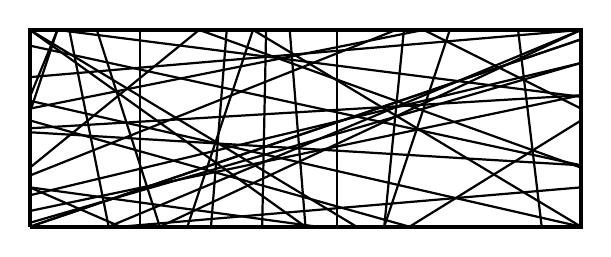
\begin{tikzpicture}[scale=0.5]
%\draw[help lines] (0,0) grid (14,5);

\draw[ultra thick] (0,0) -- (14,0) -- (14,5) -- (0,5) -- (0,0);

\draw[thick] (0,3.3) -- (0.7,5);
\draw[thick] (0,2.7) -- (9.642,0);
\draw[thick] (0,2.5) -- (14,3.34);
\draw[thick] (0,2.4) -- (14,1.56);
\draw[thick] (0,1) -- (2.3,0);
\draw[thick] (0,0) -- (14,4.76);
\draw[thick] (0,0.8) -- (14,4.16);
\draw[thick] (2.8,0) -- (2.8,5);
\draw[thick] (1.7,5) -- (3.3,0);
\draw[thick] (0,1.5) -- (4.3,5);
\draw[thick] (0,3) -- (10,5);
\draw[thick] (4,0) -- (5.66666,5);
\draw[thick] (1,5) -- (2,0);

\draw[thick] (0,2.9) -- (0.7,5);
\draw[thick] (0,3.2) -- (14,0);
\draw[thick] (0,0.4) -- (14,3.34);
\draw[thick] (0,4.6) -- (14,1.56);
\draw[thick] (0,1) -- (7.3,0);
\draw[thick] (0,0) -- (14,4.76);
\draw[thick] (0,0.1) -- (14,4.16);
\draw[thick] (7.8,0) -- (7.8,5);
\draw[thick] (0,5) -- (8.3,0);
\draw[thick] (0,1.3) -- (9.3,5);
\draw[thick] (0,3.8) -- (14,5);
\draw[thick] (9,0) -- (10.66666,5);
\draw[thick] (0,5) -- (7,0);

\draw[thick] (14,3.3) -- (0.7,5);
\draw[thick] (14,2.7) -- (9.642,0);
\draw[thick] (14,2.5) -- (14,3.34);
\draw[thick] (14,2.4) -- (14,1.56);
\draw[thick] (14,1) -- (2.3,0);
\draw[thick] (14,0) -- (14,4.76);
\draw[thick] (14,0.8) -- (14,4.16);
\draw[thick] (14,5) -- (3.3,0);
\draw[thick] (14,1.5) -- (4.3,5);
\draw[thick] (14,3) -- (10,5);
\draw[thick] (14,0) -- (5.66666,5);
\draw[thick] (14,5) -- (2,0);

\draw[thick] (7,0) -- (6.6,5);
\draw[thick] (9,0) -- (9.5,5);
\draw[thick] (13,0) -- (12.4,5);
\draw[thick] (4.6,0) -- (5,5);
\draw[thick] (5.9,0) -- (6,5);
\end{tikzpicture}
\end{center}

    \begin{itemize}
        \item More robust generalization of Pramanik and Fraser, showing that we can `thicken' or `thin' the zero set of our function with stable effects on the Hausdorff dimension of $X$.
        \pause

        \item Uncountable unions of regular sets are allowed!
    \end{itemize}
\end{frame}

\begin{frame}
    \frametitle{Applications}

    \begin{itemize}
        \item Given a subset $Y$ of $\mathbf{R}^d$ which is the countable union of sets with Minkowski dimension $\alpha$, we can find a $\mathbf{Q}$ vector subspace $X$ of $\mathbf{R}^d$ with Hausdorff dimension $d - \alpha$ disjoint from $Y$.

        \pause
        \item We can find a full dimensional subset of $\mathbf{R}^d$ avoiding the zero sets of all polynomials with rational coefficients of the form $f(y \cdot x)$ with $y \in \mathbf{Q}$. No dependence on the degree of the polynomial. Complexity is measured by rank rather than degree.

        %\pause
%        \item Given a continuous $\gamma: [0,1] \to \mathbf{R}^d$, finding $X \subset [0,1]$ such that $\gamma(x), \gamma(y), \gamma(z)$ do not form an `arithmetic progression' on the curve, in the sense that
        %
%        \[ (\gamma(x) - \gamma(y)) - (\gamma(y) - \gamma(z)) = 0 \]
        %
%        Pramanik and Fraser can avoid smooth curves. We can now avoid {\it any} curve given a Hausdorff dimension calculation. Potentially even a Hilbert curve.
    \end{itemize}
\end{frame}

\begin{frame}
    \frametitle{The Method}

    \begin{columns}

    \column{0.1\textwidth}

    \column{0.7\textwidth}
    {\Huge Two key ideas: }
    \pause

     \begin{itemize}
        \item {\Large Discretization of Scales.}
        \pause

        \item {\Large Random Disection.}
     \end{itemize}

     \end{columns}
\end{frame}

%\begin{frame}
%    \frametitle{Discretization of Scales: Intuition}

%    \begin{itemize}
%        \item {\bf Multi Scale Problem}: Find a set $X \subset \mathbf{R}$ with large Hausdorff dimension such that the base three expansion of any $x \in X$ does not contain a $1$.

        %\pause
%        \item The Cantor Set is well known to satisfy this.

        %\pause
%        \item {\bf Single Scale Problem}: Given $X_n$, find $X_{n+1}$ such that no element of $X_{n+1}$ has $1$ as the $n$'th digit in it's expansion.

        %\pause
%        \item If we solve the discrete problem for all $n$, the limiting set $X = \lim X_n$ will satisfy the multi scale problem.
%    \end{itemize}
%\end{frame}

\begin{frame}
    \frametitle{Discretization of Scales}

    \begin{figure}
        \begin{tikzpicture}[scale=4] %% Change scaling as needed

        \uncover<1->{
            \draw [|-]  (0,0) -- (4/7,0);

            \foreach \x in {1/7,2/7,3/7,4/7,5/7,6/7}
                \draw (\x,-0.5pt) -- (\x,0.5pt);

            %\foreach \x in {1,2,3}
                %\draw (\x/7, -1pt) node[anchor= north] {\tiny $\frac{\x}{N_1}$};
                %\draw (6/7, -1pt) node[anchor= north] {\tiny 1 - $\frac{1}{N_1}$};

            \draw (0,0) -- (1,0);
            \draw [-|] (6/7,0) -- (1,0) node [anchor = south west] {$X_N$};

            \foreach \x in {1/7, 3/7, 5/7,6/7}
                \draw[very thick] (\x,0) -- (\x + 1/7,0);
        }

        \uncover<2->{
            \draw [SkyBlue, very thick]  (1/7,0) -- (2/7,0);
            \draw [SkyBlue, very thick]  (3/7,0) -- (4/7,0);
            \draw [rose, very thick] (6/7+0.001,0) -- (7/7-0.001,0);

            \draw [SkyBlue, very thick] (-3/7,0.5/7) -- (-2/7,0.5/7);
            \foreach \x in {-3/7, -2/7}
                \draw (\x,0.5/7 - 0.01) -- (\x,0.5/7 + 0.01);
            \draw (-4.5/7,0.5/7) node [anchor = west] {$I_1$};

            \draw [rose, very thick] (-3/7,-0.5/7) -- (-2/7,-0.5/7);
            \foreach \x in {-3/7, -2/7}
                \draw (\x,-0.5/7 - 0.01) -- (\x, -0.5/7 + 0.01);
            \draw (-4.5/7,-0.5/7) node [anchor = west] {$I_2$};
        }


    \uncover<3->{

        \draw  (5/14,0) ellipse (1/4 and 1/16);
        \draw (13/14,0) ellipse (1/12 and 1/16);

        \def\endA{(-0.25,-0.28)}

        \draw [|-|] \endA ++(0,0) -- ++(15/14,0);

%        \draw [blue, thick] \endA  -- ++(1/7,0);
        \draw [SkyBlue, very thick] \endA  ++(0,0) -- ++(5/14,0);
        \draw [SkyBlue, very thick] \endA  ++(10/14,0) -- ++(5/14,0);
        \foreach \x in {1,...,14}
            \draw \endA  +(\x/14,-0.5pt) -- +(\x/14,0.5pt);

        \draw \endA ++(7/14,0) ellipse (10/14 and 1.5/16);





        \def\endB{(0.5,-0.5)}

        \draw [|-|] \endB ++(0,0) -- ++(5/14,0);

        \draw [rose, very thick] \endB ++(0,0) -- ++(5/14,0);

        \foreach \x in {0,...,5}
            \draw \endB  +(\x/14,-0.5pt) -- +(\x/14,0.5pt);

        \draw [SkyBlue, very thick] \endA  ++(0,0) -- ++(5/14,0);

        \draw \endB ++(2.5/14,0) ellipse (3/14 and 1.5/16);
    }

    \uncover<4-> {
        \foreach \x in {3,11}
            \draw [darkblue, very thick] \endA ++(\x/14,0) -- ++(1/14,0);
            % BlueGreen
        \draw [crimsonred, very thick] \endB ++(1/14,0) -- ++(1/14,0);

        \draw [darkblue, very thick] (1.2,-0.45) -- ++(1/7,0);
        \draw [crimsonred, very thick] (1.2,-0.6) -- ++(1/7,0);

        \foreach \x in {1.2, 1.2+1/7}
            \draw (\x,-0.45 - 0.01) -- ++(0,0.02);

        \foreach \x in {1.2, 1.2+1/7}
            \draw (\x,-0.6 - 0.01) -- ++(0,0.02);

        \draw (1,-0.45) node [anchor = west] {$J_1$};
        \draw (1,-0.6) node [anchor = west] {$J_2$};
    }

    \uncover<5->{
        \draw [|-]  (0,-0.8) -- (4/7,-0.8);

        \foreach \x in {1,...,34}
            \draw (\x/35,-0.8-0.005) -- (\x/35,-0.8+0.005);

        \foreach \x in {1,...,6}
            \draw (\x/7,-0.8-0.01) -- (\x/7,-0.8+0.01);

        \draw (0,-0.8) -- (1,-0.8);
        \draw [-|] (6/7,-0.8) -- (1,-0.8) node [anchor = north west] {$X_{N+1}$};

        \draw[very thick] (25/35,-0.8) -- (30/35,-0.8);

        \foreach \x in {8/35, 16/35, 31/35}
            \draw[very thick] (\x,-0.8) -- (\x + 1/35,-0.8);
    }
\end{tikzpicture}
    \end{figure}

    \begin{itemize}
        \item Construct $X$ as a Cantor set by limits of interval sets $X_N$.

        \pause
        \pause
        \pause
        \pause
        \pause
        \item {\bf Discrete Problem}: Given disjoint unions of length $L$ intervals $I_1, \dots, I_n$, find $J_i$ for each $i$ containing a part of each interval in $I_i$ such that $J_1 \times \dots \times J_n$ is disjoint from $Z$.
    \end{itemize}
\end{frame}

\begin{frame}
    \frametitle{Queueing}

    \begin{itemize}
        \item Using a queueing procedure, and performing this single scale procedure over all arbitrarily fine covers $I_1, \dots, I_n$ of the set $X$ gives a fractal avoiding set $X$.

        \pause
        \item {\bf Reason}: If we consider distinct $x_1, \dots, x_n \in X$, there are intervals $I_1, \dots, I_n$ with $x_1 \in I_1, \dots, x_n \in I_n$ considered at some scale. Then $x_1 \in J_1, \dots, x_n \in J_n$, and so $(x_1, \dots, x_n) \in J_1 \times \dots \times J_n$ cannot be contained in $Z$.
    \end{itemize}
\end{frame}

\begin{frame}
    \frametitle{Exploiting Randomness}

    \begin{figure}
        \begin{tikzpicture}[scale=3] %% Change scaling as needed
            \draw [|-|]  (0,0) -- (6/7,0);
            \draw [|-|] (-1/7,1/7) -- (-1/7,7/7);

            \draw[dashed] (0,1/7) -- (0,2/7) -- (1/7,2/7) -- (1/7,3/7) -- (0,3/7) -- (0,4/7) -- (1/7,4/7) -- (2/7,4/7) -- (2/7,5/7) -- (2/7,6/7) -- (1/7,6/7) -- (1/7,1) -- (2/7,1) -- (3/7,1) -- (3/7,6/7) -- (3/7,5/7) -- (3/7,4/7) -- (3/7,3/7) -- (2/7,3/7) -- (2/7,2/7) -- (4/7,2/7) -- (4/7,3/7) -- (5/7,3/7) -- (5/7,2/7) -- (6/7,2/7) -- (6/7,1/7) -- (0,1/7);

            \draw[dashed] (6/7,7/7) -- (5/7,7/7) -- (5/7,6/7) -- (6/7,6/7) -- (6/7,7/7);

            \draw (6/7,0) node [anchor = south west] {$I_1$};
            \draw (-1/7,7/7) node [anchor = south east] {$I_2$};
            \draw (1.1,1) node [anchor = south east] {$Z$};

            \foreach \x in {2,4}
                \draw (\x/7,-0.5pt) -- (\x/7,0.5pt);

            \foreach \x in {3,5}
                \draw (-1/7,\x/7) ++(-0.5pt,0) -- ++(1pt,0);

%            \foreach \x in {1,...,6}
%                \draw (\x/7,-0.5pt) -- (\x/7,0.5pt);

            \foreach \x in {2,...,6}
                \draw (-1/7,\x/7) ++(-0.5pt,0) -- ++(1pt,0);

            \foreach \x in {1,...,5}
                \draw (\x/7,-0.5pt) -- (\x/7,0.5pt);

            \draw [|-|]  (0,0) -- (6/7,0);
            \draw [|-|] (-1/7,1/7) -- (-1/7,7/7);

            \draw[dashed] (0,1/7) -- (0,2/7) -- (1/7,2/7) -- (1/7,3/7) -- (0,3/7) -- (0,4/7) -- (1/7,4/7) -- (2/7,4/7) -- (2/7,5/7) -- (2/7,6/7) -- (1/7,6/7) -- (1/7,1) -- (2/7,1) -- (3/7,1) -- (3/7,6/7) -- (3/7,5/7) -- (3/7,4/7) -- (3/7,3/7) -- (2/7,3/7) -- (2/7,2/7) -- (4/7,2/7) -- (4/7,3/7) -- (5/7,3/7) -- (5/7,2/7) -- (6/7,2/7) -- (6/7,1/7) -- (0,1/7);

            \draw[dashed] (6/7,7/7) -- (5/7,7/7) -- (5/7,6/7) -- (6/7,6/7) -- (6/7,7/7);

            \draw (6/7,0) node [anchor = south west] {$I_1$};
            \draw (-1/7,7/7) node [anchor = south east] {$I_2$};
            \draw (1.1,1) node [anchor = south east] {$Z$};

            \foreach \x in {2,4}
                \draw (\x/7,-0.5pt) -- (\x/7,0.5pt);

            \foreach \x in {3,5}
                \draw (-1/7,\x/7) ++(-0.5pt,0) -- ++(1pt,0);

%            \foreach \x in {1,...,6}
%                \draw (\x/7,-0.5pt) -- (\x/7,0.5pt);

            \foreach \x in {2,...,6}
                \draw (-1/7,\x/7) ++(-0.5pt,0) -- ++(1pt,0);

            \foreach \x in {1,...,5}
                \draw (\x/7,-0.5pt) -- (\x/7,0.5pt);
\end{tikzpicture}
    \end{figure}

    \begin{itemize}
        \item How do we prove the discrete scale argument?
        %\pause

        \pause
        \item Aside from $Z$'s dimension, we have little structural knowledge.
        %\pause

        \pause
        \item Random choices of the $J_k$ avoid $Z$ effectively.

        %\pause
        \item We obtain for all but $o(1)$ of the length $L$ intervals in $I_k$, $J_k$ contains a length $L^\beta$ section of each, where $\beta = d(nd - \alpha)/(n - 1)$. This ratio gives the Hausdorff dimension bound $(nd-\alpha)/(n-1)$ for $X$.
    \end{itemize}
\end{frame}

\begin{frame}
    \frametitle{Conclusion}

    {\Huge So What's Next?}
\end{frame}

\begin{frame}
    \frametitle{Extension to Hausdorff Dimension}

    \begin{itemize}
        \item There is no obvious reason why our techniques should fail when $Z$ has {\it Hausdorff dimension} $\alpha$ rather than a Minkowski dimension bound.

        \pause
        \item We are trying to use hyperdyadic coverings rather than coverings at a single scale to achieve this.
    \end{itemize}
\end{frame}

\begin{frame}
    \frametitle{Analogies with Hypergraphs}

    \begin{figure}
    \begin{subfigure}{.6\textwidth}
        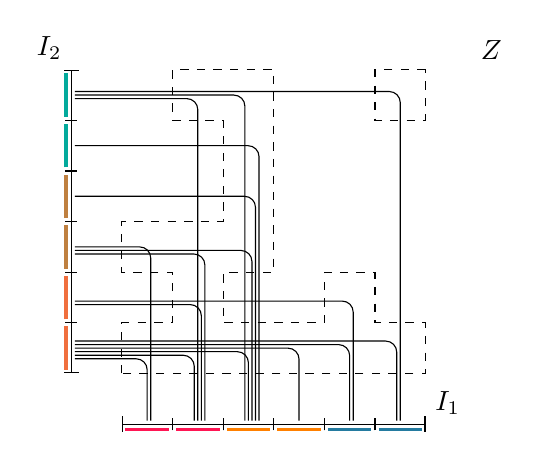
\begin{tikzpicture}[scale=4.5] %% Change scaling as needed
            \uncover<1->{
            \draw [|-|]  (0,0) -- (6/7,0);
            \draw [|-|] (-1/7,1/7) -- (-1/7,7/7);

            \draw[dashed] (0,1/7) -- (0,2/7) -- (1/7,2/7) -- (1/7,3/7) -- (0,3/7) -- (0,4/7) -- (1/7,4/7) -- (2/7,4/7) -- (2/7,5/7) -- (2/7,6/7) -- (1/7,6/7) -- (1/7,1) -- (2/7,1) -- (3/7,1) -- (3/7,6/7) -- (3/7,5/7) -- (3/7,4/7) -- (3/7,3/7) -- (2/7,3/7) -- (2/7,2/7) -- (4/7,2/7) -- (4/7,3/7) -- (5/7,3/7) -- (5/7,2/7) -- (6/7,2/7) -- (6/7,1/7) -- (0,1/7);

            \draw[dashed] (6/7,7/7) -- (5/7,7/7) -- (5/7,6/7) -- (6/7,6/7) -- (6/7,7/7);

            \draw (6/7,0) node [anchor = south west] {$I_1$};
            \draw (-1/7,7/7) node [anchor = south east] {$I_2$};
            \draw (1.1,1) node [anchor = south east] {$Z$};

            \foreach \x in {2,4}
                \draw (\x/7,-0.5pt) -- (\x/7,0.5pt);

            \foreach \x in {3,5}
                \draw (-1/7,\x/7) ++(-0.5pt,0) -- ++(1pt,0);

%            \foreach \x in {1,...,6}
%                \draw (\x/7,-0.5pt) -- (\x/7,0.5pt);
            }

            \uncover<2-> {
            \foreach \x in {2,...,6}
                \draw (-1/7,\x/7) ++(-0.5pt,0) -- ++(1pt,0);

            \foreach \x in {1,...,5}
                \draw (\x/7,-0.5pt) -- (\x/7,0.5pt);
            }

            \uncover<3-> {

            \draw[rounded corners] (11/14,0.01) -- (11/14,13/14+0.01) -- (-1/7+0.01,13/14+0.01);
            \draw[rounded corners] (5/14-0.01,0.01) -- (5/14-0.01,13/14) -- (-1/7+0.01,13/14);
            \draw[rounded corners] (3/14,0.01) -- (3/14,13/14-0.01) -- (-1/7+0.01,13/14-0.01);

            \draw[rounded corners] (11/14-0.01,0.01) -- (11/14-0.01,3/14+0.02) -- (-1/7+0.01,3/14+0.02);
            \draw[rounded corners] (9/14,0.01) -- (9/14,3/14+0.01) -- (-1/7+0.01,3/14+0.01);
            \draw[rounded corners] (7/14,0.01) -- (7/14,3/14) -- (-1/7+0.01,3/14);
            \draw[rounded corners] (5/14,0.01) -- (5/14,3/14-0.01) -- (-1/7+0.01,3/14-0.01);
            \draw[rounded corners] (3/14-0.01,0.01) -- (3/14-0.01,3/14-0.02) -- (-1/7+0.01,3/14-0.02);
            \draw[rounded corners] (1/14,0.01) -- (1/14,3/14-0.03) -- (-1/7+0.01,3/14-0.03);

            \draw[rounded corners] (3/14+0.01,0.01) -- (3/14+0.01,5/14-0.02) -- (-1/7+0.01,5/14-0.02);
            \draw[rounded corners] (9/14+0.01,0.01) -- (9/14+0.01,5/14-0.01) -- (-1/7+0.01,5/14-0.01);

            \draw[rounded corners] (1/14+0.01,0.01) -- (1/14+0.01,7/14) -- (-1/7+0.01,7/14);
            \draw[rounded corners] (3/14+0.02,0.01) -- (3/14+0.02,7/14-0.02) -- (-1/7+0.01,7/14-0.02);
            \draw[rounded corners] (5/14+0.01,0.01) -- (5/14+0.01,7/14-0.01) -- (-1/7+0.01,7/14-0.01);

            \draw[rounded corners] (5/14+0.02,0.01) -- (5/14+0.02,9/14) -- (-1/7+0.01,9/14);
            \draw[rounded corners] (5/14+0.03,0.01) -- (5/14+0.03,11/14) -- (-1/7+0.01,11/14);
            }

            \uncover<4-> {
                \foreach \x in {0,1}
                    \draw [deepred, very thick] (\x/7+0.01,-0.015) -- (\x/7+1/7-0.01,-0.015);

                \foreach \x in {2,3}
                    \draw [orange, very thick] (\x/7+0.01,-0.015) -- (\x/7+1/7-0.01,-0.015);

                \foreach \x in {4,5}
                    \draw [deepblue, very thick] (\x/7+0.01,-0.015) -- (\x/7+1/7-0.01,-0.015);

                \foreach \x in {1,2}
                    \draw [deeporange, very thick] (-1/7-0.015, \x/7+0.01) -- (-1/7-0.015,\x/7 + 1/7-0.01);

                \foreach \x in {3,4}
                    \draw [brown, very thick] (-1/7-0.015, \x/7+0.01) -- (-1/7-0.015,\x/7 + 1/7-0.01);

                \foreach \x in {5,6}
                    \draw [JungleGreen, very thick] (-1/7-0.015, \x/7+0.01) -- (-1/7-0.015,\x/7 + 1/7-0.01);
            }
\end{tikzpicture}
\end{subfigure}%
\begin{subfigure}{.4\textwidth}
            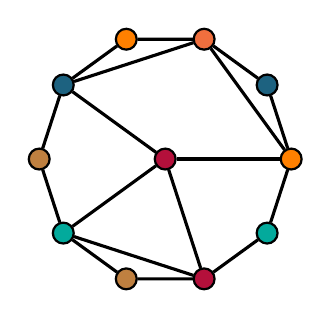
\begin{tikzpicture}[every node/.style={circle,thick,draw,scale=0.8}, line width=0.04cm, scale=0.8]
    \uncover<5-> {
    \node[fill = {rgb:red,255;green,22;blue,84}] (K) at (0:0) {};

    \node[fill = orange] (E) at (0:2) {};
    \node[fill = {rgb:red,36;green,123;blue,160}] (J) at (36:2) {};
    \node[fill = deeporange] (A) at (72:2) {};
    \node[fill = orange] (F) at (108:2) {};
    \node[fill = {rgb:red,36;green,123;blue,160}] (B) at (144:2) {};
    \node[fill = brown] (G) at (180:2) {};
    \node[fill = JungleGreen] (C) at (216:2) {};
    \node[fill = brown] (H) at (252:2) {};
    \node[fill = {rgb:red,255;green,22;blue,84}] (D) at (288:2) {};
    \node[fill = JungleGreen] (I) at (324:2) {};

    \draw (A) -- (B);
    \draw (A) -- (F);
    \draw (F) -- (B);
    \draw (B) -- (G);
%    \draw (B) -- (C);
    \draw (G) -- (C);
    \draw (C) -- (H);
    \draw (C) -- (D);
    \draw (H) -- (D);
    \draw (D) -- (I);
%    \draw (D) -- (E);
    \draw (I) -- (E);
    \draw (E) -- (A);
    \draw (E) -- (J);
    \draw (J) -- (A);
%    \draw (K) -- (A);
    \draw (K) -- (B);
    \draw (K) -- (C);
    \draw (K) -- (D);
    \draw (K) -- (E);
    }
        \end{tikzpicture}
        \end{subfigure}
    \end{figure}

    \begin{itemize}
        \pause
        \pause
        \pause
        \pause
        \item The Discrete Scale problem can be viewed as finding an independent set in a hypergraph containing each color.

        \pause
        \item We are looking to using other methods on hypergraphs to improve the bound when $Z$ has certain structural properties (like for the low rank result).
    \end{itemize}
\end{frame}

\begin{frame}
    \frametitle{Interested in Learning More?}

    \begin{itemize}
            \item Read Keleti (1999) for a simple use of scale discretization on a particular configuration avoidance problem.
            \pause
            \item Read M\'{a}th\'{e} (2012) for a construction where $f$ is assumed to be a polynomial of bounded degree.
            \pause
            \item Read Pramanik and Fraser (2016) for a general construction where $f$ is smooth and nonsingular. We generalize their work.
            \pause
            \item Read Josh's, Malabika, and my paper if it's ever published...
    \end{itemize}

    Thanks for listening!
\end{frame}

\end{document}